\documentclass{beamer}
\usepackage[francais]{babel}
\usepackage[utf8]{inputenc}
\usepackage{cclicenses}
\usepackage{csquotes} %guillemets
\usepackage{graphicx}
\usepackage[bars]{beamerthemetree} %Beamer theme v 2.2
\usepackage{mathtools}

\usetheme{Warsaw}
\usecolortheme{seahorse}

\setbeamertemplate{navigation symbols}{}


\AtBeginSubsection[]
{
  \begin{frame}
    \frametitle{Table des matières}
    \tableofcontents[
  currentsection,
  sectionstyle=show/show,
  subsectionstyle=show/shaded/hide
]
  \end{frame}
}

\title[Introduction à GNU/Linux
\hspace{25mm} \insertframenumber/\inserttotalframenumber]
{Introduction aux systèmes Unix-like et aux commandes Shell}% (optional, only for long titles)
\author[Jean-Philippe Eisenbarth et Quentin Laporte-Chabasse] % (optional, for multiple authors)
{}
\institute[Telecom Nancy, Université de Lorraine] % (optional)
{
  Telecom Nancy, Université de Lorraine
}
\date{\today} % (optional)
{}
\subject{Informatique}

\begin{document}


    \begin{frame}
      \titlepage

      \begin{center}
        {\scriptsize \centerline{\href{http://creativecommons.org/licenses/by-sa/4.0/}{Licence Creative Commons 
Attribution-ShareAlike 4.0 International}}}
        \bysa{}
      \end{center}
    \end{frame}
    
    \frame{\tableofcontents}
    
    \section[De Unix à GNU/Linux]{De Unix à GNU/Linux}
    
        \subsection[Les débuts avec Unix]{Les débuts avec Unix}
        
            \begin{frame}
                \frametitle{De Unix à GNU/Linux}
                \framesubtitle{Les débuts avec Unix}
                \begin{itemize}
                    \item Unix est l'un des premiers systèmes d'exploitation
                    \item Début de la conception et implémentation en 1969 par Ken Thompson, Dennis Ritchie, Douglas McIloy, Joe Ossanna qui travaillent pour les laboratoires Bell.
                    \item Sorti en 1971
                    \item 1975 : distribution du code source aux universités à des fins éducatives, moyennant l'achat d'une licence.
                \end{itemize}
            \end{frame}
            
            \begin{frame}[t]{\insertsubsectionhead}
                \frametitle{De Unix à GNU/Linux}
                \framesubtitle{Les débuts avec Unix}
                \begin{itemize}
                    \item 1977 : Apparition d'une des premières variantes, BSD (Berkeley Software Distribution).
                    \item Les Unix-like se répandent rapidement dans les milieux académiques.
                    \item 1987 : Apparition de Minix, destiné à l'éducation.
                    \item 1999 : Apparition de Mac OS X, un système dérivé de FreeBSD (un Unix-like)
                \end{itemize}
            \end{frame}
            
            \begin{frame}
                \frametitle{De Unix à GNU/Linux}
                \framesubtitle{L'arborescence de fichiers avec Unix}
                \begin{figure}[h]
                  \centering
                  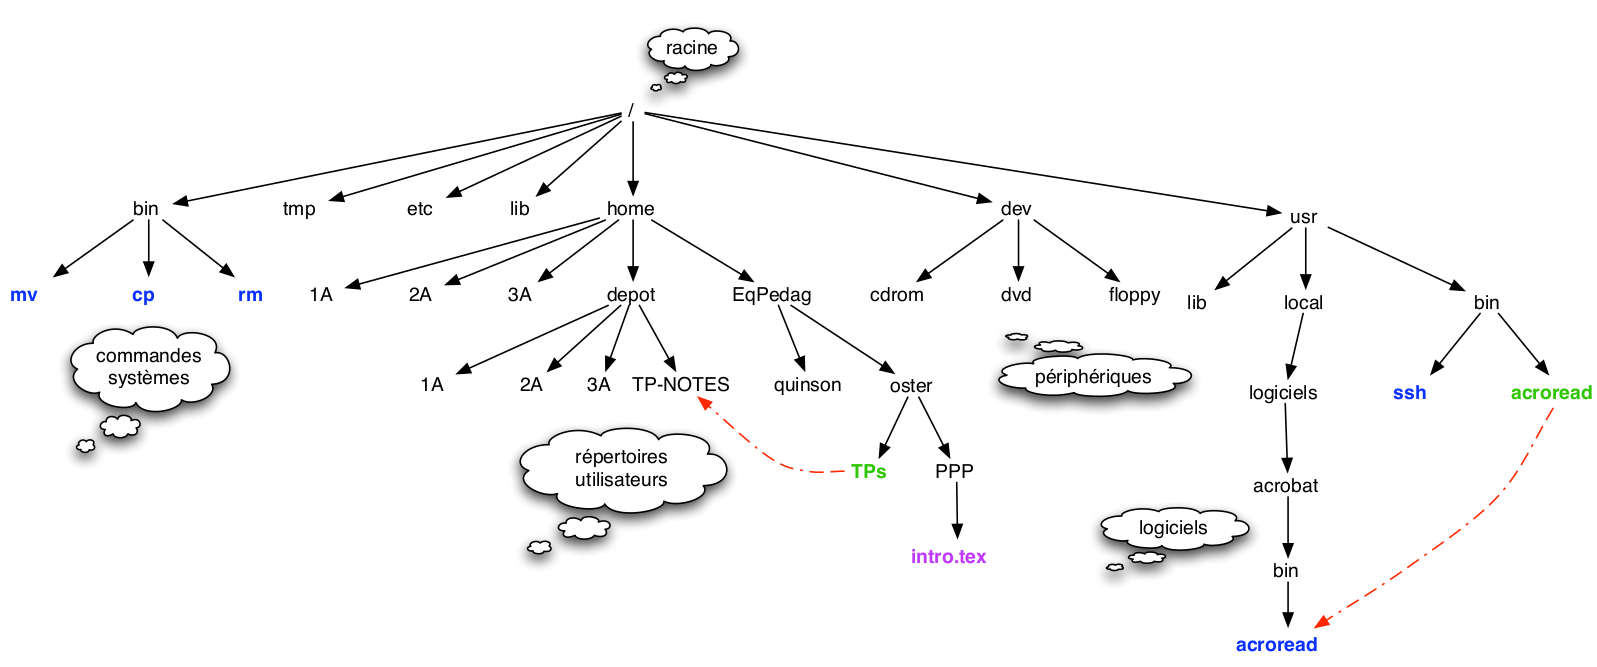
\includegraphics[scale=0.208]{figures/filesystem_unix.png}
                \end{figure}
                \tiny{Auteur : M. Gerald Oster}
            \end{frame}
            
        \subsection[Le projet Linux]{Le projet Linux}
        
            \begin{frame}
                \frametitle{De Unix à GNU/Linux}
                \framesubtitle{Le projet Linux}
                \begin{itemize}
                    \item 1991 : Linus Torvalds, alors étudiant à l'université d'Helsinki, commence à travailler sur un noyau qu'il appelera plus tard \foreignquote{french}{Linux}.
                    \item Association de Linux et des applications de Minix pour créer un système d'exploitation complet.
                \end{itemize}
            \end{frame}
            
        \subsection[Le projet GNU]{Le projet GNU}
        
            \begin{frame}
                \frametitle{De Unix à GNU/Linux}
                \framesubtitle{Le projet GNU}
                \begin{itemize}
                    \item 1983 : Richard Stallman commence le projet GNU avec pour but de créer un système libre compatible Unix.
                    \item 1985 : Création de la \textit{Free Software Foundation} qui a pour but de promouvoir le logiciel \foreignquote{french}{libre}.
                \end{itemize}
            \end{frame}
            
            \begin{frame}
                \frametitle{De Unix à GNU/Linux}
                \framesubtitle{Les quatre libertés fondamentales}
                Un logiciel est considéré comme libre, selon la définition de la \textit{Free Software Foundation} s'il respecte ces quatre libertés fondamentales :
                \begin{itemize}
                    \item n\degres0 : la liberté d'exécuter le programme, pour tous les usages ;
                    \item n\degres1 : la liberté d'étudier le fonctionnement du programme et de l'adapter à ses besoins ;
                    \item n\degres2 : la liberté de redistribuer des copies du programme;
                    \item n\degres3 : la liberté d'améliorer le programme et de distribuer ces améliorations au public, pour en faire profiter toute la communauté.
                \end{itemize}
            \end{frame}
        
       \subsection[Le système d'exploitation GNU/Linux]{Le système d'exploitation GNU/Linux}
        
            \begin{frame}
                \frametitle{De Unix à GNU/Linux}
                \framesubtitle{GNU/Linux}
                \begin{itemize}
                    \item Au final, GNU était composé de beaucoup de logiciels mais un noyau manquait pour en faire un système d'exploitation.
                    \item Linus Torvalds décide alors de faire de Linux un logiciel libre afin de pouvoir intégrer les logiciels du projet GNU : GNU/Linux est né.
                    \item De nombreuses distributions sont alors apparues : Debian (1993), Archlinux (2002), Fedora (2003), Ubuntu(2004), ...
                \end{itemize}
            \end{frame}
    
    \section[Quelques commandes Shell utiles]{Quelques commandes Shell utiles}
    
       \begin{frame}
            \frametitle{Quelques commandes Shell utiles}
            \framesubtitle{Différence entre option et argument}
            Une option est une valeur que prend la commande pour modifier son effet/son exécution.
            
            Un argument est une valeur sur laquelle la commande s'exécute (une entrée du programme).       
        \end{frame}
    
        \subsection[Commandes de manipulation de répertoires et fichiers]{Commandes de manipulation de répertoires et fichiers}
    
            \begin{frame}
                \frametitle{Quelques commandes Shell utiles}
                \framesubtitle{ls - list directory contents}
                La commande \foreignquote{french}{ls} permet de lister l'ensemble des fichiers du répertoire courant.
                Options courantes :
                \begin{itemize}
                    \item \foreignquote{french}{-l} : affiche selon un formatage \foreignquote{french}{long}
                    \item \foreignquote{french}{-a} : affiche également les fichiers cachés
                \end{itemize}
            \end{frame}
            
            \begin{frame}
                \frametitle{Quelques commandes Shell utiles}
                \framesubtitle{cd - change the shell working directory}
                La commande \foreignquote{french}{cd} change le répertoire courant
            \end{frame}
        
            \begin{frame}
                \frametitle{Quelques commandes Shell utiles}
                \framesubtitle{touch - change file timestamps}
                La commande \foreignquote{french}{touch} permet de changer les dates d'accès et de modification d'un fichier ou en créer un nouveau s'il n'existe pas.
            \end{frame}
         
            \begin{frame}
                \frametitle{Quelques commandes Shell utiles}
                \framesubtitle{mkdir - make directories}
                La commande \foreignquote{french}{mkdir} Permet de créer un répertoire
                
                Une option courante est \foreignquote{french}{-p} qui permet de créer les répertoires qui n'existent pas dans le chemin passé en paramètre.
            \end{frame}
            
            \begin{frame}
                \frametitle{Quelques commandes Shell utiles}
                \framesubtitle{mv - move (rename) files}
                La commande \foreignquote{french}{mv} permet de déplacer un fichier.
                
                Prend deux arguments sous forme de chemins :
                    \begin{itemize}
                        \item la source, qui sera déplacée
                        \item la destination, là où sera copiée la source
                    \end{itemize}
                    
                Si le chemin de la source et de la destination est le même (seul le nom de fichier change) alors la commande renomme le fichier.
            \end{frame}
            
            \begin{frame}
                \frametitle{Quelques commandes Shell utiles}
                \framesubtitle{cp - copy files and directories}
                La commande \foreignquote{french}{cp} Permet de copier des fichiers ou des répertoires.
                
                Prend deux arguments sous forme de chemins :
                    \begin{itemize}
                        \item la source, qui sera copiée
                        \item la destination, là où sera copié la source
                    \end{itemize}
            \end{frame}
            
            \begin{frame}
                \frametitle{Quelques commandes Shell utiles}
                \framesubtitle{rm - remove files or directories}
                La commande \foreignquote{french}{rm} permet d'effacer des fichiers ou des répertoires.
                
                Options courantes :
                \begin{itemize}
                    \item \foreignquote{french}{-r} : efface un répertoire et tout son contenu ;
                    \item \foreignquote{french}{-i} : demande confirmation pour chaque fichier ; 
                \end{itemize}
            \end{frame}
            
            \begin{frame}
                \frametitle{Quelques commandes Shell utiles}
                \framesubtitle{chmod - change file mode bits}
                Cette commande permet de changer les droits d'un fichier.
                
                Elle peut s'utiliser de deux manières :
                \begin{itemize}
                    \item \foreignquote{french}{chmod MODE file}, le mode verbeux
                    \item \foreignquote{french}{chmod OCTAL-MODE file}, le mode octal
                \end{itemize}
                
                Voir le TP pour de plus amples explications.
            \end{frame}
        
        \subsection[Commandes de lecture de fichiers]{Commandes de lecture de fichiers}
        
            \begin{frame}
                \frametitle{Quelques commandes Shell utiles}
                \framesubtitle{cat - concatenate files and print on the standard output}
                La commande \foreignquote{french}{cat} permet d'afficher entièrement le contenu d'un fichier dans la sortie standard.
            \end{frame}
            
            \begin{frame}
                \frametitle{Quelques commandes Shell utiles}
                \framesubtitle{less - opposite of more}
                Permet de lire le contenu d'un fichier.
            \end{frame}
             
        \subsection[Commandes d'écriture dans des fichiers]{Commandes d'écriture dans des fichiers}
        
            \begin{frame}
                \frametitle{Quelques commandes Shell utiles}
                \framesubtitle{echo - display a line of text}
                La commande \foreignquote{french}{echo} permet d'afficher l'argument passé sur la sortie standard.
                
                Elle s'utilise généralement avec une redirection de sortie.
            \end{frame}
                
            \begin{frame}
                \frametitle{Quelques commandes Shell utiles}
                \framesubtitle{echo et redirections de sortie}
                Exemple : echo "bonjour" $>$ file.txt
                
                Cette commande redirige le résultat de la commande \foreignquote{french}{echo} dans le fichier \foreignquote{french}{file.txt} en écrasant ce qui s y trouvait précédemment.
                
                Pour rediriger sans écraser (i.e. ajout à la suite du fichier), il faut utiliser \foreignquote{french}{$>>$}.
            \end{frame}
        
        \subsection[Commandes diverses]{Commandes diverses}
        
            \begin{frame}
                \frametitle{Quelques commandes Shell utiles}
                \framesubtitle{man - format and display the on-line manual pages}
                La commande \foreignquote{french}{man} permet de consulter un manuel de référence.
                
                Dans son utilisation courante cette commande attend un argument qui est la commande dont on veut lire la documentation.
                
            \end{frame}
            
            \begin{frame}
                \frametitle{Quelques commandes Shell utiles}
                \framesubtitle{man - format and display the on-line manual pages}
                \foreignquote{french}{Man} possède plusieurs sections.
                
                On peut obliger \foreignquote{french}{man} à ne chercher que dans une section particulière en passant le numéro de celle-ci juste avant l'argument.
                
                Sinon lors de la recherche d'une commande il recherchera linéairement dans toutes les sections jusqu'à trouver la page qui documente la commande en argument.
            \end{frame}
            
            \begin{frame}
                \frametitle{Quelques commandes Shell utiles}
                \framesubtitle{man - format and display the on-line manual pages}
                Exemple : man 1 ls
                
                Pour voir l'ensemble des sections, il suffit de consulter la page man de man en tapant \foreignquote{french}{man man}.
            \end{frame}
% etc
\end{document}